\section{Experimental Validation}
\label{S:Exp}

In this section we present how we made our data set and the results using the two algorithms.



\newcommand{\multiplier}{7.25cm}
\begin{figure*}[th]
\centering
\subfigure[Pure Odometry]{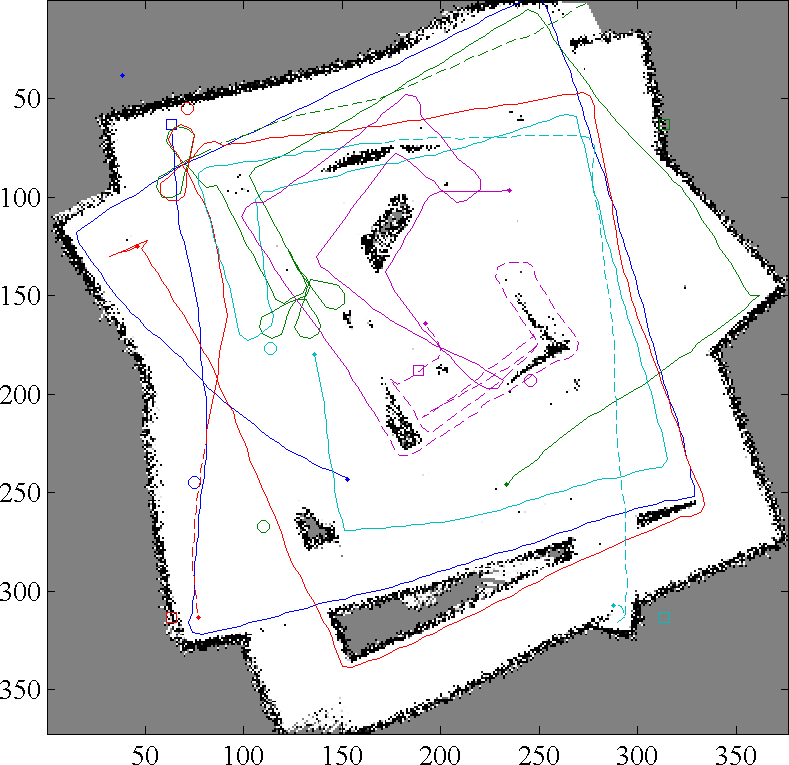
\includegraphics[width=\multiplier]{../FinalFigures/PureOdometry}}
\subfigure[Known Poses]{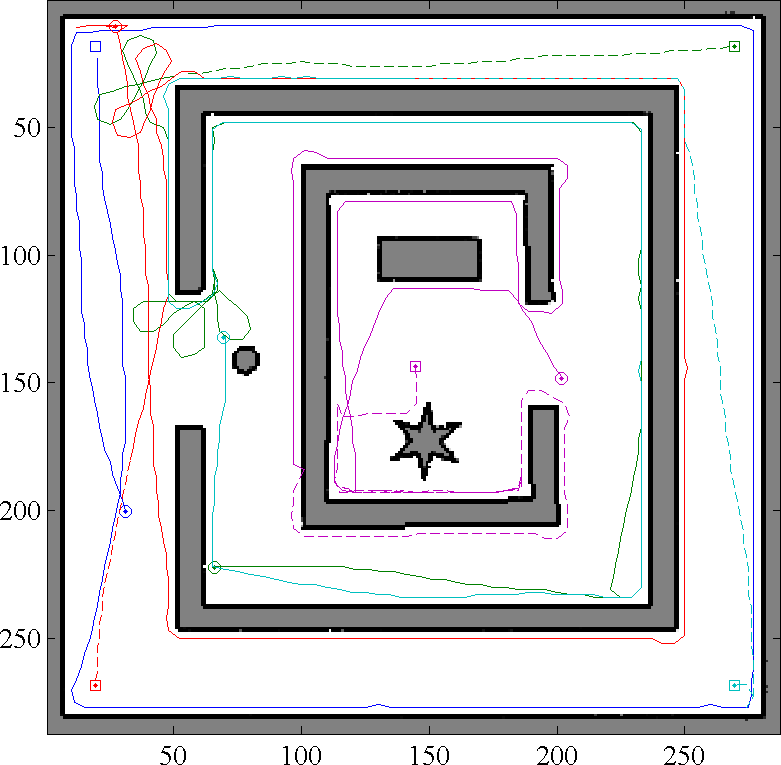
\includegraphics[width=\multiplier]{../FinalFigures/KnownPoses}}\\
\subfigure[Howard Implementation: Unknown Poses, low noise.]{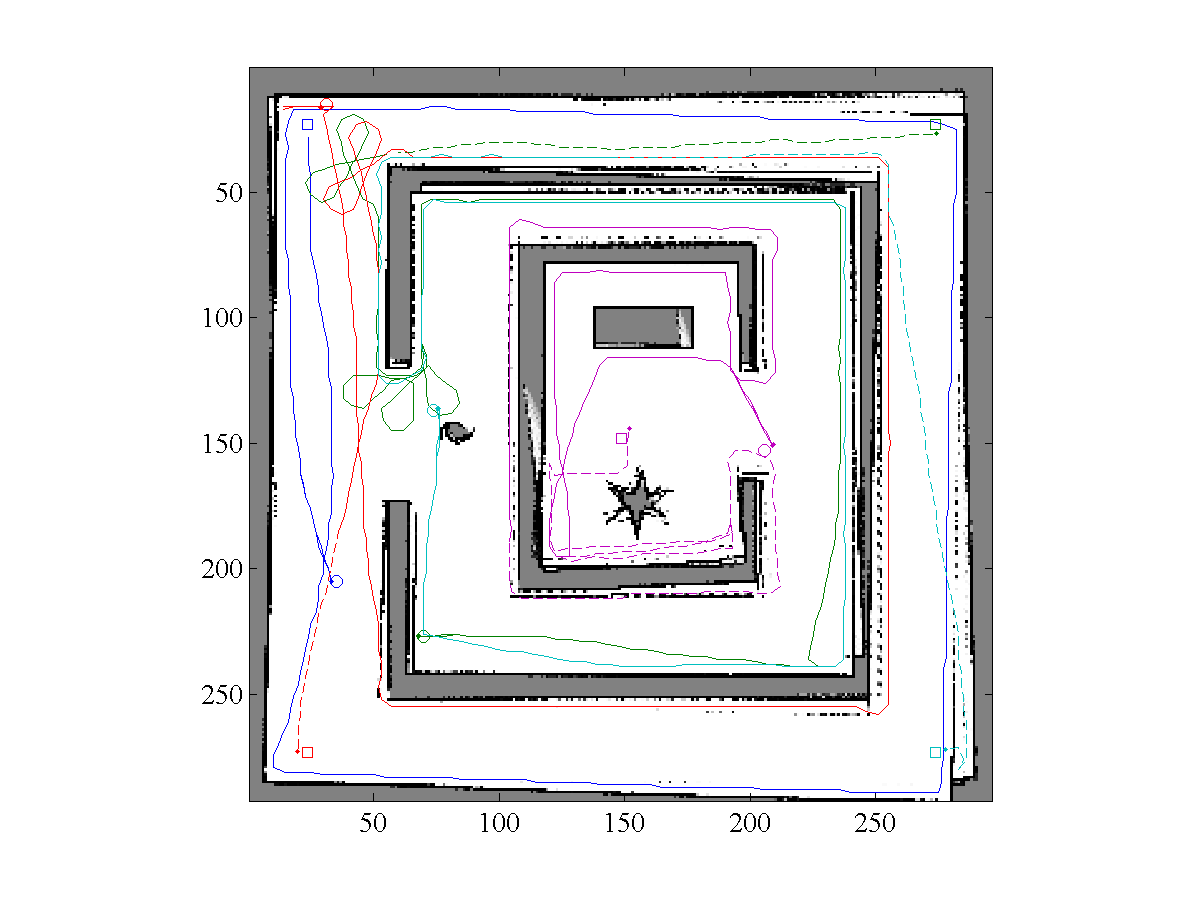
\includegraphics[width=\multiplier]{../FinalFigures/HowardLowNoise}}
\subfigure[Proposed Implementation: Unknown Poses, low noise.]{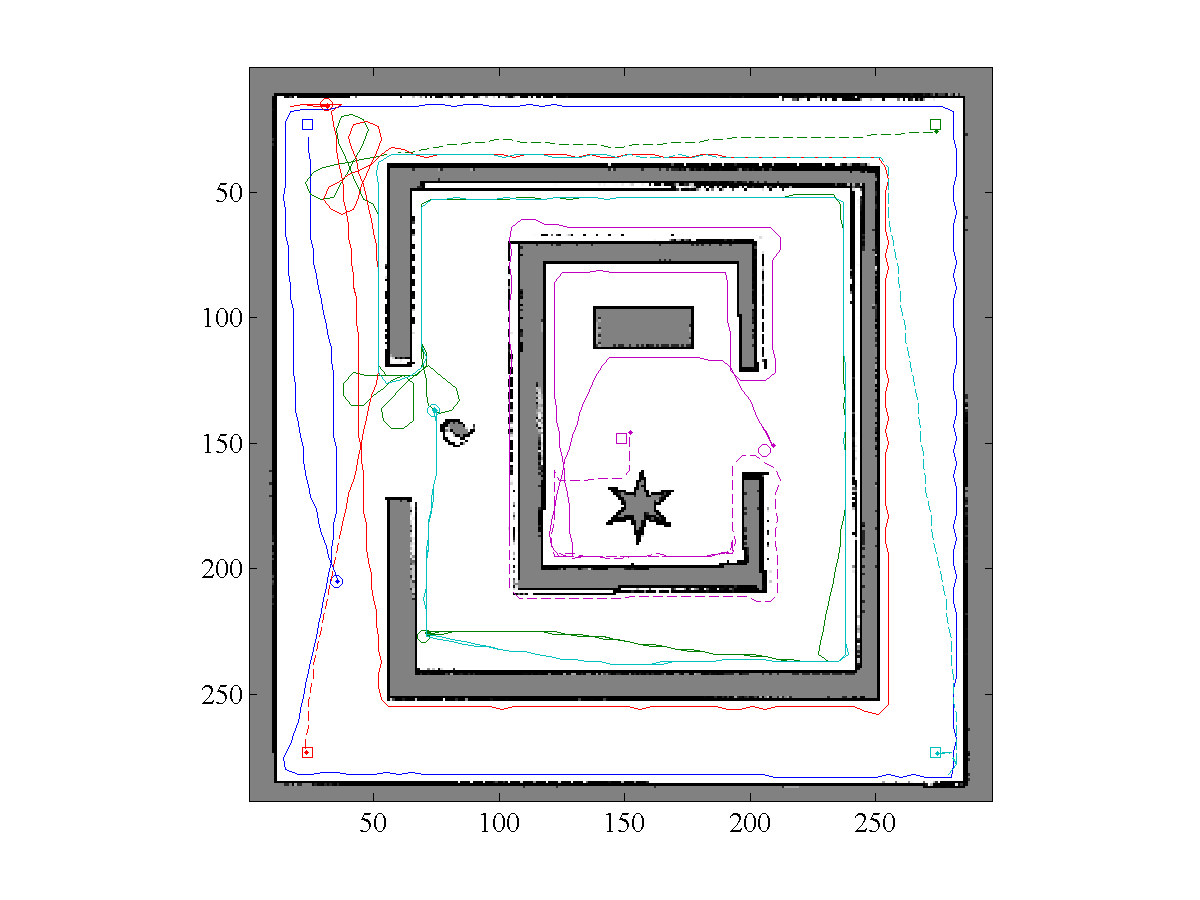
\includegraphics[width=\multiplier]{../FinalFigures/OursLowNoise}}\\
\subfigure[Howard Implementation: Unknown Poses, High noise.]{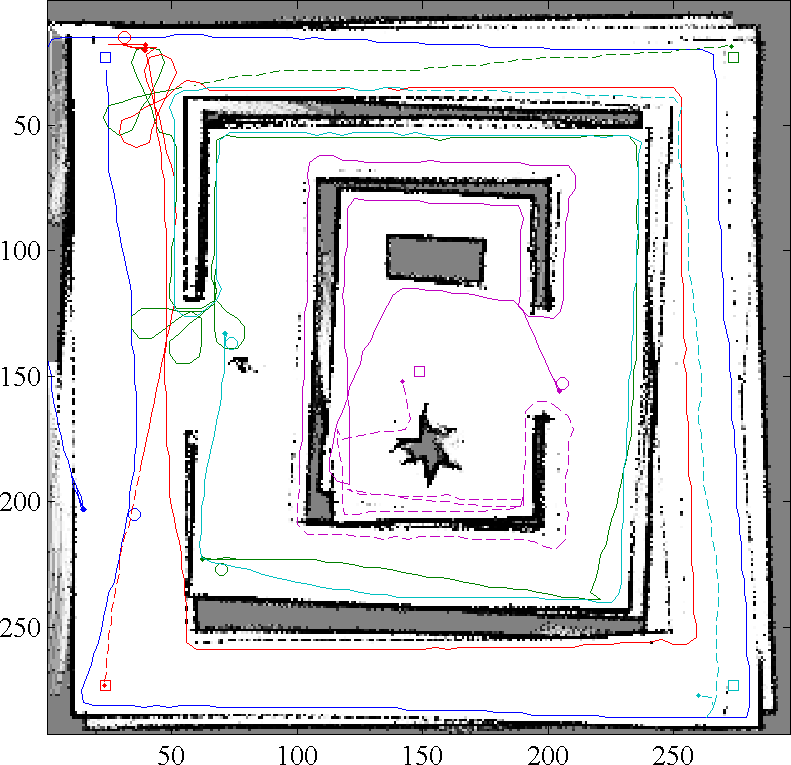
\includegraphics[width=\multiplier]{../FinalFigures/HowardHighNoise}}
\subfigure[Proposed Implementation: Unknown Poses, High noise.]{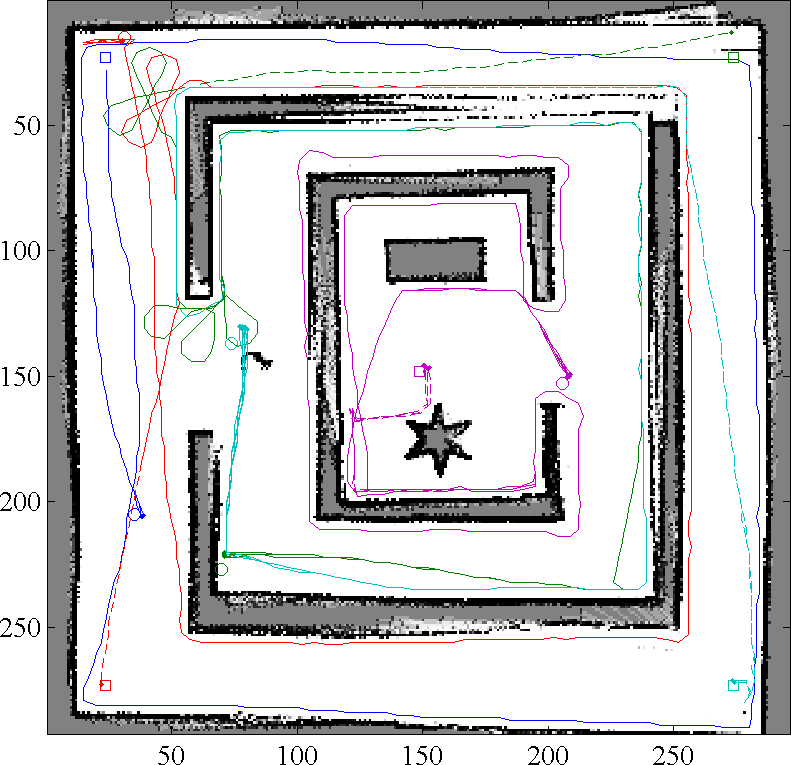
\includegraphics[width=\multiplier]{../FinalFigures/OursHighNoise}}
\caption{Comparison between Howard's implementation and the proposed implementation.}
\label{fig:Comp}
\end{figure*}



\subsection{The Data Set}
\label{S:Exp:DataSet}

The data set consists of PAS triple $(\textbf{x}^i_t,u^i_t,z^i_t)$, where $i$ denotes the robot ID, and $t$ denotes the time.  The pose, $x^i_t$, is comprised of the $x_t^i$-$y^i_t$ position, as well as the orientation $\theta^i_t$.  The input, $u^i_t$, is composed of the position deflection, $\delta^i_t$, and the angular deflection, $\omega_t$.  Finally, the measurements, $z^i_t$, contains scan data for rays cast out at $1^\circ$ intervals from $[-90^\circ,90^\circ]$, to simulate a laser scan.  

To obtain the measurements we use a ray-circle intersection algorithm.

\subsubsection{Ray-Circle Intersection}

The scan data is constructed using ray-circle intersection of a binary image, $I$ (like that of Fig. \ref{subfig:Enc} without the paths).  The idea of ray-circle intersection is to find all the object pixels within a region of interest (ROI), in this case the shaded pixels in the semi-circle, $I_{semi}$, as seen in Fig. \ref{subfig:raycirc}, 
\begin{equation}
I_{semi}=\left\{I_{xy}\in I |\  ||I_xy-I_{\textbf{x}_t^i}||_2^2<r^2 \right\},
\label{eq:Isemi}
\end{equation}
where $I_{\textbf{x}_t^i}$ is the position of the robot $i$ in the map.

Then $I_{semi}$ is intersected with the object, $I_{obj}={I_{xy}\in I | \ I_{xy}=1}$ (the filled squares in Fig. \ref{subfig:raycirc}, to get $I_{filled}$.  A ray is then defined by 
\begin{equation}
\textbf{v}_k=\begin{bmatrix}
I_{x_t^i}+r_k^j \cos(\phi_k)\\
I_{y_t^i}+r_k^j \sin(\phi_k)\\
\end{bmatrix}, 
\label{eq:ray}
\end{equation}
where $r_k^j>0$ is some partitioning of the length of the ray up to the maximum range of the sensor.  This ray is intersected with $I_{filled}$ to get $I_{ray}$ (colored in orange in Fig. \ref{subfig:raycirc}).  Finally, the minimum distance to the object, $r_{k}^*$ , is selected (the $r_k^j$ corresponding the blue square in Fig. \ref{subfig:rstar}) to get the distance measurement $z_t^{i,k}$ of the object to the robot.  

\begin{equation}
r_k^*=\min_{j} r_{k}^j
\end{equation}


\begin{figure}[ht]
\centering
\subfigure[$I_{filled}$ and the intersection with the ray $\textbf{v}_k$.]{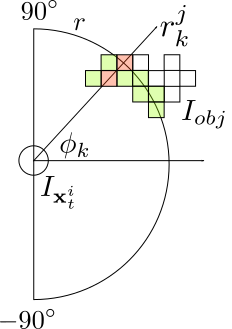
\includegraphics[height=4cm]{../FinalFigures/RayCircleIntersection1}\label{subfig:raycirc}}
\subfigure[The selection of $r_k^*$.]{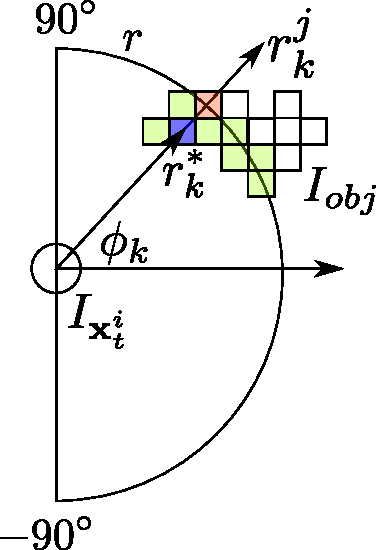
\includegraphics[height=4cm]{../FinalFigures/RayCircleIntersection}\label{subfig:rstar}}
\caption{Visualization of Ray-Circle Intersection}
\label{fig:raycirc}
\end{figure}

We introduce zero mean, additive Gaussian noise with variance $Q$ to $z_t^{i,k}$ to get noisy measurements $\hat{z}_t^{i,k}$:
\begin{equation}
\hat{z}_t^{i,k}=z_t^{i,k}+\mathcal{N}(0,Q).
\end{equation}

\subsubsection{Wall Following}

In this paper we will use wall following to search the environment.  The specifics of this implementation are that it is turned on when $t\in[50,200]$, each robot is equipped with a parity bit to ensure that some robots move in opposite directions, and if the robot happens to get stuck in a loop, wall following will temporarily turn off.

Using wall following to search the environment led to the choice of the odometry motion model, because wall following can be easily implemented with scan data obtained using ray-circle intersection.


\subsubsection{The Odometry Motion Model}

The motion model used was the classic odometry motion model.  
\begin{equation}
\begin{bmatrix}
x_{t}\\
y_{t}\\
\theta_{t}
\end{bmatrix}=\begin{bmatrix}
x_{t-1}\\
y_{t-1}\\
\theta_{t-1}
\end{bmatrix}+\begin{bmatrix}
\hat{\delta}_{t-1}  \cos(\theta_t+\hat{\omega}_t)\\
\hat{\delta}_{t-1}\sin(\theta_t+\hat{\omega}_t)\\
\hat{\omega}_{t-1}
\end{bmatrix},
\label{eq:OdometryMotion}
\end{equation}
where
\begin{eqnarray}
\hat{\delta}_{t-1}&=&\delta_{t-1}-\mathcal{N}(0,\alpha_1\delta_{t-1}^2+\alpha_2\omega_{t-1}^2)\\
\hat{\omega}_{t-1}&=&\omega_{t-1}-\mathcal{N}(0,\alpha_3\delta_{t-1}^2+\alpha_4\omega_{t-1}^2).
\end{eqnarray}

The reverse odometry model is
\begin{equation}
\begin{bmatrix}
x_{t-1}\\
y_{t-1}\\
\theta_{t-1}
\end{bmatrix}=\begin{bmatrix}
x_{t}\\
y_{t}\\
\theta_{t}
\end{bmatrix}-\begin{bmatrix}
\hat{\delta}_t  \cos(\theta_t-\hat{\omega}_{t-1})\\
\delta_{t}\sin(\theta_t-\hat{\omega}_{t-1})\\
\hat{\omega}_{t-1}
\end{bmatrix}
\label{eq:ReverseOdometryMotion}
\end{equation}

\subsubsection{Encounter Detection and Relative Pose}

In place of using a hypothetical camera to determine if robot encounters occur, we use the ray-circle intersection algorithm.  We treat each robot as an object in the binary image, $I$, and if a $(r_k^*,\phi_k)$ is found to coincide with an added robot, and encounter is declared and a relative pose is calculated.  



\subsubsection{The Environment, Robot Trajectories, and Encounters}

Fig. \ref{fig:EnvEnc} contains the test environment and the time when each encounter occurred.  Fig. \ref{subfig:Encvst} shows at what time a robot encountered another, note: only the first encounter is used.

Fig. \ref{subfig:Enc} shows the binary map of the environment, the paths each robot took (colored lines), the point when a robot encounter occurred (dashed gray lines), and where the encounter occurred (thick grey line).
the path each robot took, when a robot encountered another robot, 

\begin{figure}[ht]
\centering
\subfigure[Robot encounters versus time.]{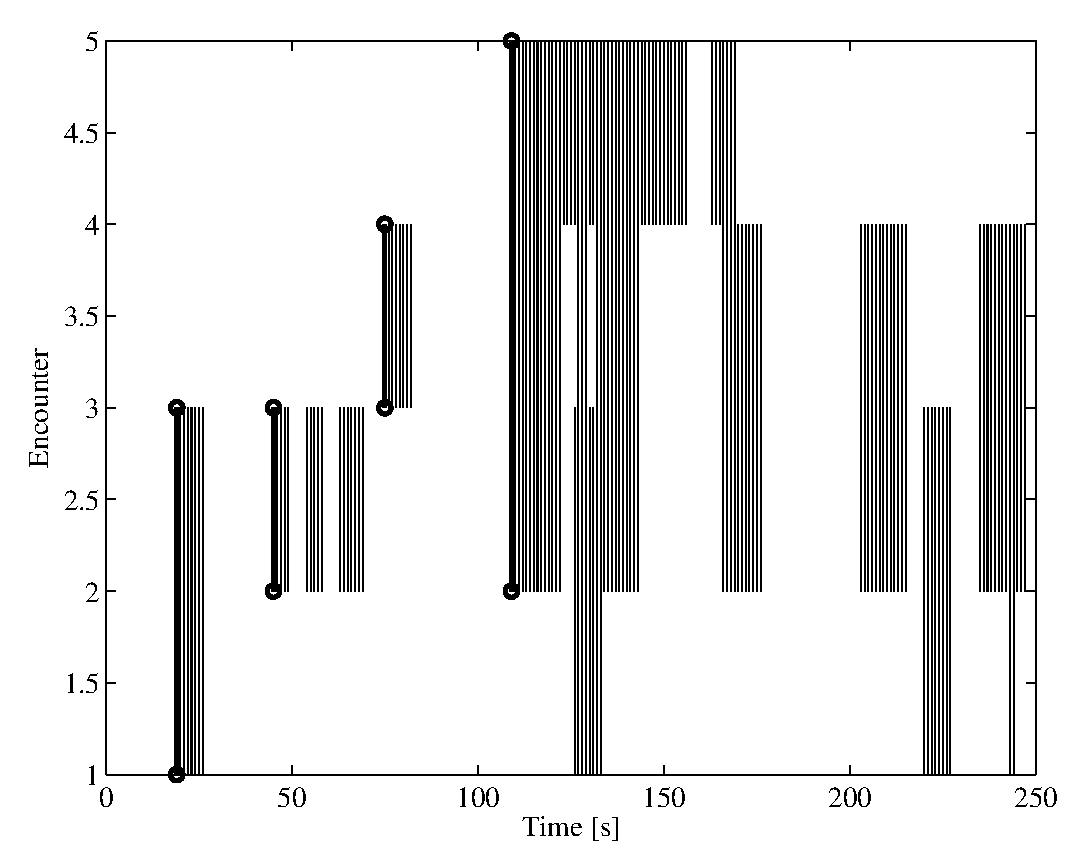
\includegraphics[width=\columnwidth]{../FinalFigures/EncountersTimes}\label{subfig:Encvst}}
\subfigure[The test geometry, robot paths (colored lines), and encounters (dashed gray lines).]{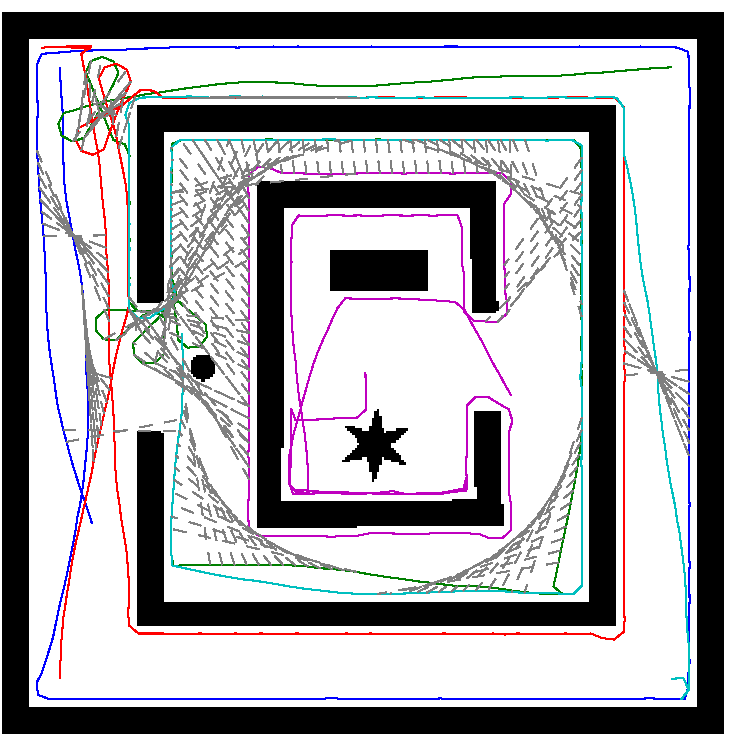
\includegraphics[width=\columnwidth]{../FinalFigures/Encounters}\label{subfig:Enc}}
\caption{Environment geometry, robot paths, and encounters.}
\label{fig:EnvEnc}
\end{figure}








\subsection{The Results}
\label{S:Exp:DataSet}






